\section{System Design}

\begin{figure*}[h]
    \centering
      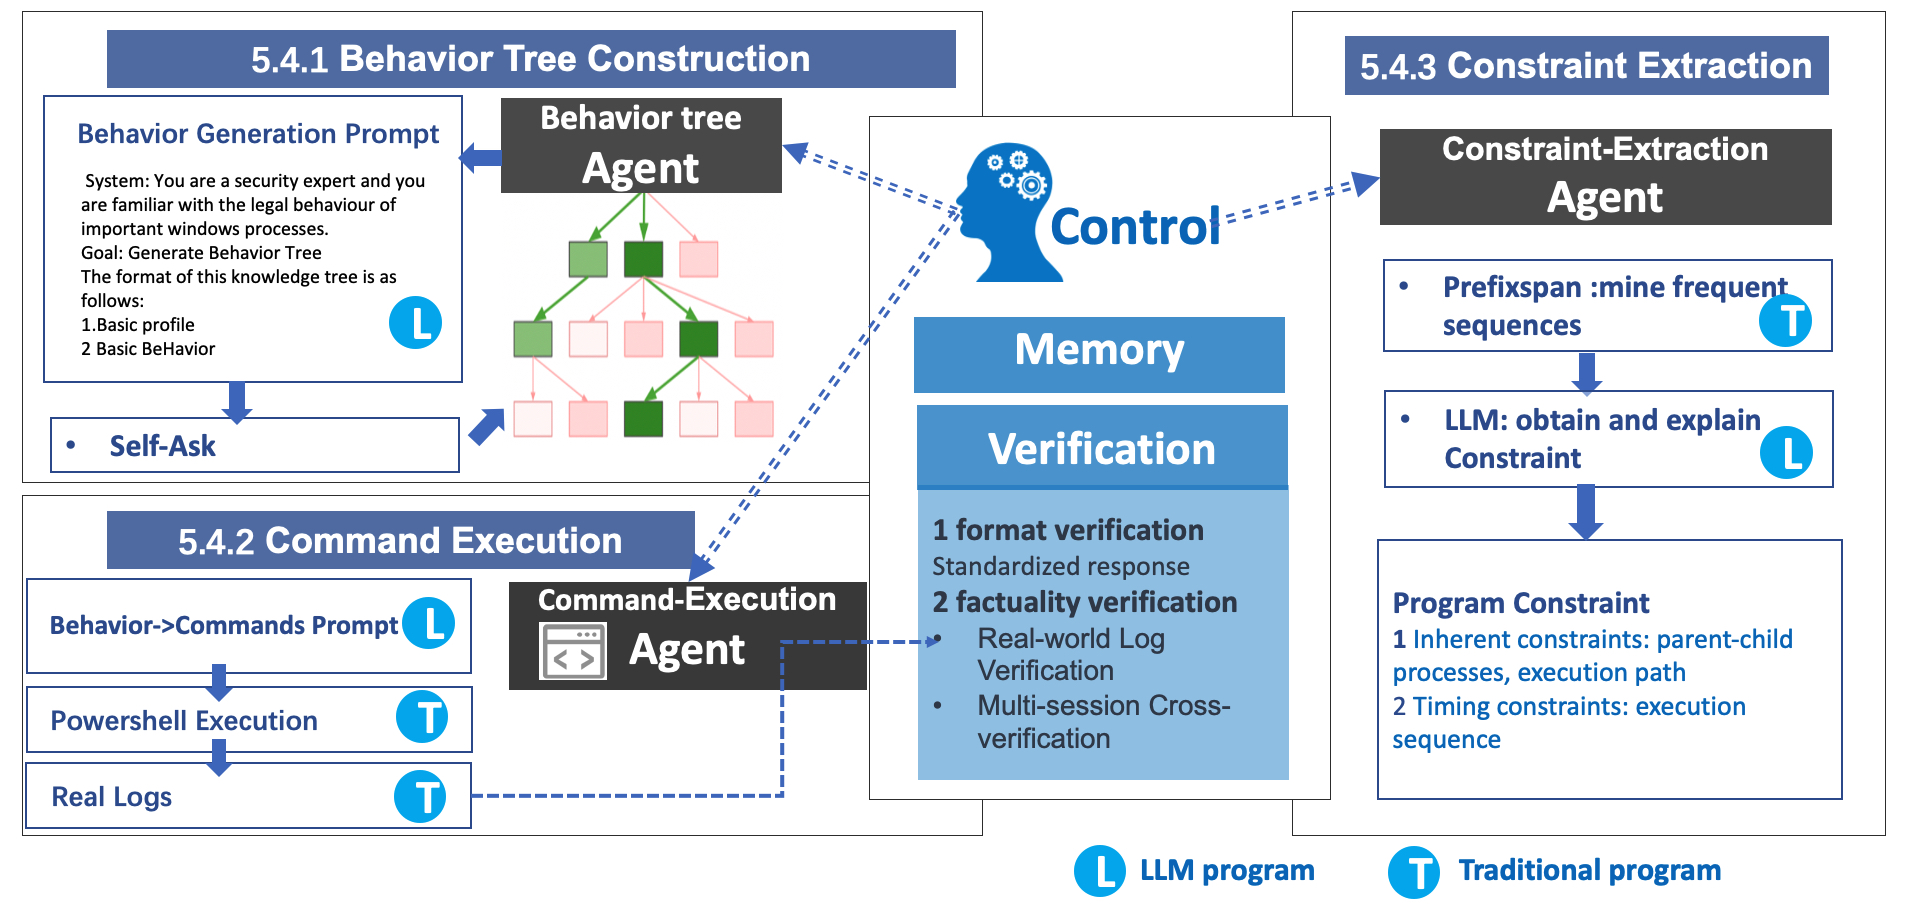
\includegraphics[width=1\textwidth]{figs/prompt.jpg}
    \caption{Profile Construction Framework: Our system leverages a central "controller" equipped with memory storage and validation capabilities. Guided by this controller, we employ three key modules: 1) Behavior Tree Construction Module, focused on mapping out behavioral patterns; 2) Command Execution Module, designed for active process deployment; and 3) Log Constraint Extraction Module, responsible for deducing log-based regulations. Collaboratively, these units harness a blend of LLM-assisted strategies and traditional techniques to meticulously craft program profiles.}
    \label{fig-framework}
    \end{figure*}

\subsection{Definitions}

\subsubsection{System Entity and System Event}
We consider the following four types of system entities: Processes, Files, Registry, and Network Connections (i.e., sockets). A system event $e = (src, dst, rel, time)$ models an interaction between two system entities, where $src$ is the source entity, $dst$ is the destination entity, $rel$ denotes the relationship between them (e.g., a process writing into a file), and $time$ is the timestamp when the event occurred. Please note that, in a system event, only process entities can be the source entities. Each system entity is associated with a set of attributes. For example, a process entity has attributes such as its pid and executable path. We display the entity attributes and relationships that we consider in Table 1.

\subsubsection{System Provenance Graph}
Consider a process $p$ in the system, identified by its process id and host. The system provenance graph, also referred to as the dependency graph, of $p$ is defined as the graph that includes all system entities with either control dependencies (i.e., starting or ending processes) or data dependencies (i.e., reading or writing processes) related to $p$. Formally, we define the provenance graph of $p$ as $G(p) =< V, E >$, where $V$ and $E$ denote the sets of vertices and edges, respectively. In this case, vertices $V$ correspond to system entities, while edges $E$ are indicative of system events.


\subsection{Process Monitoring}

The Process Monitoring is crucial: we must gather logs from various system processes. To achieve this, we employ Windows' robust log collection and processing tool, Sysmon, for comprehensive system log capture. Using its default configuration, Sysmon ensures maximal log collection. 

However, given the vast volume of logs, it becomes imperative to trim down the data. Leveraging expert knowledge, we streamline the logs by removing redundant and mundane events.
\subsubsection{Noisy Events Reduction}
The low-level and verbose nature of audit logs makes the presence of noisy events one of the primary challenges analysts struggle with.

\textbf{Redundant events.}
In behavior instances, there are events when removed that do not change the data transfers. We incorporate domain knowledge in to enhance redundant event reduction.

\textbf{Mundane events.}
Another source of noise comes from file operations that are regularly performed for an action.
Then, given sequences of events for each program, we summarize events always occurring in a fixed pattern as mundane events. Essentially, we formulate the mundane event identification problem as the longest common subsequence (LCS) searching problem. Given event sequences of a program, we extract the LCS among them as the mundane events.

\subsection{Process Classification}
We crafted a prompt to query the LLM regarding the existence of a program by its name. Based on the LLM's response, we categorized these processes into three distinct categories: legitimate process names, illegitimate process names, and uncertain process names (owing to the inherent incompleteness of the GPT database). For processes falling under the legitimate category, we proceed to construct their profiles using the methods detailed in the subsequent sections. For the latter two categories, we flag them as potentially malicious, warranting further investigation by security analysts.

\subsection{Profile Construction}

Addressing the challenges highlighted in the prior section, we present our solution, ProCon, designed to construct program profiles by leveraging the combined strength of LLM-driven modules.

At the heart of ProCon lies a central control unit, often referred to as the "brain". Within this brain are two integral components: the memory and the validation mechanisms, the latter comprising both format verification and factual verification. Factual verification relies on real-log validation and inter-session cross-checking among multiple LLM sessions.
This central control brain orchestrates the operations of three distinct agent modules: the Behavior Tree Construction Module, the Command Execution Module, and the Log Constraint Extraction Module. Each of these modules manages its own LLM session and context, ensuring both coherence and specialized expertise.
These agent modules embody a harmonious blend of LLM-driven processes (like behavior tree construction) and conventional computational tasks (like frequent sequence mining). Operating under the guidance of the central brain, these traditional and LLM-driven processes collaborate seamlessly, working in tandem to autonomously craft detailed program profiles.




\subsubsection{Behavior Tree Construction}

For every program, our objective was to capture as many behaviors as possible. To achieve this, we crafted a behavior tree that comprehensively describes actions. Moreover, to augment this tree and unearth additional behaviors, we employed a "self-ask" pattern where the LLM, based on its current knowledge tree, formulates questions and furnishes corresponding answers. When the number of behaviors exceeds memory constraints, we employed a memory management mechanism, caching the results in an in-memory database.

\begin{figure*}[h]
    \centering
    \begin{subfigure}{0.48\textwidth}
      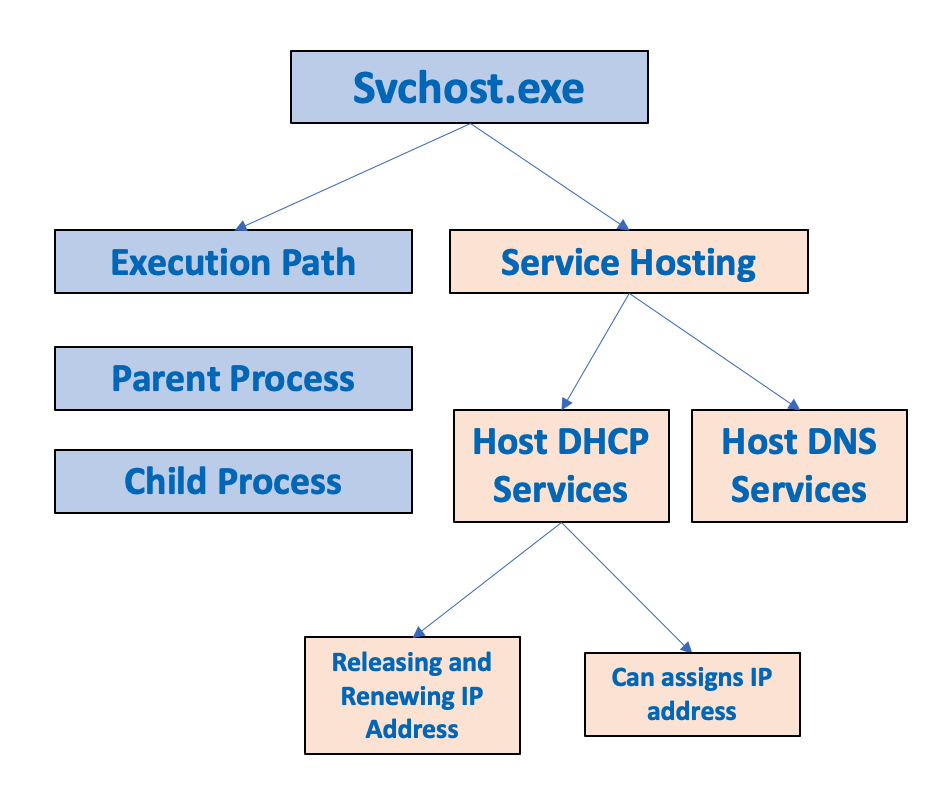
\includegraphics[width=1\textwidth]{figs/tree1.jpg}
      \caption{Behavior Tree Representation}
    \end{subfigure}
    \begin{subfigure}{0.48\textwidth}
    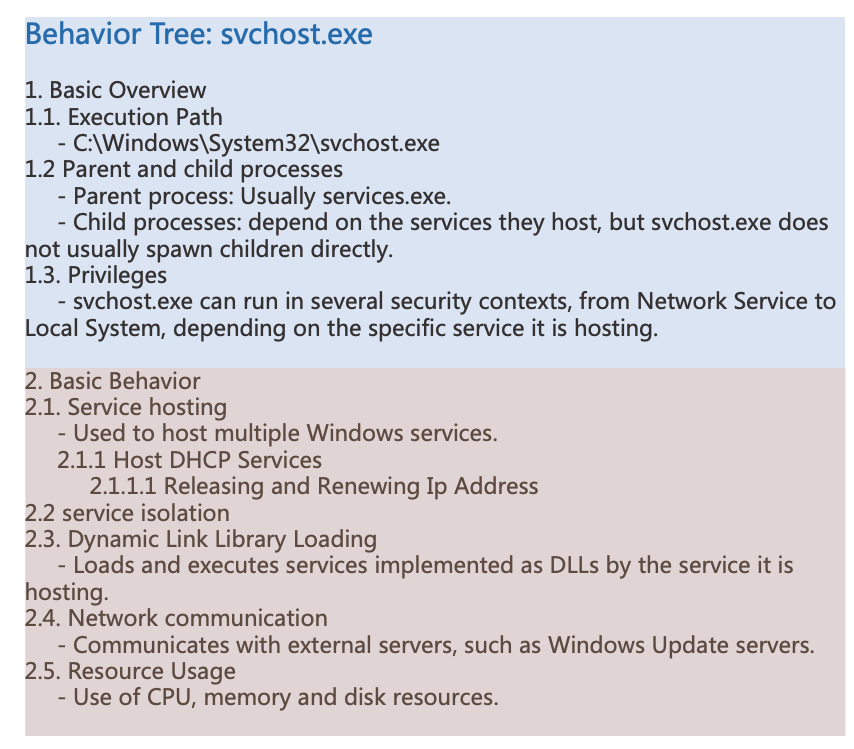
\includegraphics[width=1\textwidth]{figs/tree2.jpg}
    \caption{Behavior Tree Representation in natural Language}
    \end{subfigure}
    \vspace{-0.05in}
    \caption{Behavior Tree in a) visualized tree format, and b) natural language format encoded in LLM.}
    \label{fig-framework}
    \vspace{-0.15in}
    \end{figure*}

\begin{definition}[Behavior Tree]
A Behavior Tree (BT) is a tuple \((N, B)\), where:
\begin{enumerate}
    \item \(N\) is a set of nodes organized in a tree structure. Each node represents a legitimate behavior of a program. Every node possesses a unique identifier with a special node, called the root, which lacks a parent. Except for the root, each node has precisely one parent and zero or more children. These children nodes can represent sub-behaviors.
    \item \(B\) is a function that assigns to each node \(n \in N\) a set of attributes \(B(n)\). Each attribute is a pair \((b, w)\), where \(b\) is the behavior name and \(w\) is a description or attribute of that behavior. The set of attributes may vary for different nodes.
\end{enumerate}
The parent node represents the program's name, while child nodes depict the natural language descriptions of various behaviors.
\end{definition}

\begin{itemize}
    \item \textbf{Initial Behavior Tree Construction}: Using a preliminary prompt, we establish a rudimentary Behavior Tree (BT) structure. This prompt delineates the objective, role, desired output format for the behavior tree, as well as several executable commands. 
    \item \textbf{Automatic Behavior Generator}: It prompts continuous questions to extend behaviors grounded on the present behavior tree. This tool, through a self-querying approach, facilitates the generation of additional behaviors.
    \item \textbf{Behavior Tree Update}: Post session, it's essential to revitalize the knowledge tree with the insights garnered.
    \item \textbf{Termination}: The "Finish" command serves as an indicator that all objectives have been met. Args include a "response" parameter that offers a final response, notifying the user of the completion of objectives.
\end{itemize}

Then, responses from the LLM undergo a twofold verification process:
\begin{itemize}
\item Format Verification: Ensures the output aligns with the predefined structure.
\item Factual Verification: Assesses the accuracy and validity of the content. 
\end{itemize}
Lastly, this refined structure integrates the new information regarding token limitations and the vector database used for memory storage.


\subsubsection{Command Execution}
To operationalize behaviors, we leaned heavily on the LLM. Behaviors identified as translatable were scripted into actionable Powershell commands using the LLM. For behaviors that resisted direct translation into executable commands, we cataloged them for future reference, with the aim of tapping into the LLM's vast knowledge at a later stage.
To streamline this process, we initiated the task with a prompt: "I'll provide you with a description of the program's behavior. Can you generate the corresponding Powershell executable commands?" However, we found the direct application of this prompt yielded suboptimal results.

To refine and guide the model's output, we incorporated the Chain of Thought (COT) approach by prompting the LLM to "Make sure to reason step by step". Furthermore, furnishing specific examples served as additional guidance, helping us to obtain more precise and actionable commands from the model.
This structure aims to describe the iterative and guided approach used to extract actionable commands from the LLM effectively.

\subsubsection{Constraint Extraction}
For inherent program constraints, such as execution paths and parent-child process relationships, the LLM could readily provide answers. Validating these answers was straightforward, requiring only log collection and analysis from the system.

When dealing with temporal sequence constraints, we employed the prefixspan sequence mining algorithm to unveil intricate relationships amongst logs. Rather than directly probing the LLM for this knowledge, we strategically presented it with established relationships and then sought its insights on the sequence and interplay of these logs. This indirect inquiry approach endowed us with both enhanced accuracy and depth in the model's responses.

Given a set of log sequences \( \mathcal{D} \), where each sequence \( S \) contains multiple logs \( L \), and each log is a tuple \( (s, o, d) \) consisting of a source process \( s \), an operation \( o \), and a destination \( d \), the goal is to extract frequent subsequences \( \mathcal{F} \) that exceed a given threshold \( \theta \).
\begin{itemize}
    \item \( \mathcal{D} \) - A set of log sequences.
    \item \( S \) - A sequence in \( \mathcal{D} \) containing multiple logs.
    \item \( L \) - A log in \( S \), represented as a tuple.
    \item \( (s, o, d) \) - A tuple representing each log, where:
    \begin{itemize}
        \item \( s \) - The source process.
        \item \( o \) - The operation.
        \item \( d \) - The destination or object of the operation.
    \end{itemize}
    \item \( \mathcal{F} \) - The set of frequent subsequences.
    \item \( \theta \) - The threshold value.
\end{itemize}


\begin{algorithm}
\caption{Frequent Subsequence Mining from Log Sequences}
\begin{algorithmic}[1]
\Require A set of log sequences \( \mathcal{D} \), threshold \( \theta \)
\Ensure Frequent subsequences \( \mathcal{F} \)
\Function{PrefixSpanMining}{$\mathcal{D}$, $\theta$}
    \State $\mathcal{F} \gets \emptyset$
    \For{each $S$ in $\mathcal{D}$}
        \For{each log $L$ in $S$}
            \If{\Call{support}{$L$, $\mathcal{D}$} $\geq \theta$}
                \State $\mathcal{F}$.add($L$)
                \State $projectedDB \gets$ \Call{project}{$\mathcal{D}$, $L$}
                \State $\mathcal{F} \gets \mathcal{F} \cup$ \Call{PrefixSpanMining}{$projectedDB$, $\theta$}
            \EndIf
        \EndFor
    \EndFor
    \State \Return $\mathcal{F}$
\EndFunction
\Statex
\Function{support}{log, $\mathcal{D}$}
    \State $count \gets 0$
    \For{each $S$ in $\mathcal{D}$}
        \If{log is a subsequence of $S$}
            \State $count \gets count + 1$
        \EndIf
    \EndFor
    \State \Return $count$
\EndFunction
\Statex
\Function{project}{$\mathcal{D}$, log}
    \State $projectedDB \gets \emptyset$
    \For{each $S$ in $\mathcal{D}$}
        \If{log is a subsequence of $S$}
            \State append the part of $S$ after log to $projectedDB$
        \EndIf
    \EndFor
    \State \Return $projectedDB$
\EndFunction
\end{algorithmic}
\end{algorithm}


\subsection{Verification}

To ensure the authenticity and accuracy of the information obtained from GPT, considering the potential biases or misconceptions of machine learning models, we have adopted two core validation strategies:

\begin{itemize}
    \item Multi-session Cross-validation: By initiating multiple independent sessions, we cross-reference the answers provided by GPT. This ensures the consistency of the model's responses across different contexts. If there are significant discrepancies in the answers obtained from multiple inquiries, we have reason to doubt their accuracy, prompting further investigation or verification.
    \item External Knowledge Source Validation: In order to verify the authenticity of the answers from GPT, we trace back the source of the information, referencing authoritative and reliable external materials for verification. This method not only bolsters our confidence in the answers but also offers a deeper and more comprehensive understanding.
\end{itemize}

Throughout this procedure, validating the LLM's outputs for accuracy was paramount. Beyond real-world execution validation, the entire process incorporated multiple sessions for cross-validation purposes.
In essence, our methodology offers a fully automated approach, enabling swift construction of new program profiles. At its core, our technique embodies a mechanism where the LLM engages in self-criticism, ensures self-consistency, and continually evolves, making it a dynamic, self-reflective, and adaptive system for automatic program profiling.


\subsection{Threat Detection}

This forms the foundation of our offline process for building individual process profiles. For online detection, when confronted with processes that have random or obfuscated names, an initial query is made to GPT to ascertain the existence of said process. If it is determined that the process does not exist, it is highly probable that it is malicious. Processes that do exist but are not available in our knowledge base are further profiled using our established methodology.


For the process of anomaly detection, we leverage a plethora of rules derived from the preceding steps, with validation methods suited for both local and real-world industrial scenarios. In the context of local validation, these rules are scripted in a Python-parseable format, enabling Python-based evaluations to ascertain whether inherent constraint rules and temporal constraint rules are violated.

For industrial application, we transcribe these rules into query statements compatible with Splunk and Azure platforms. This allows for seamless integration into industrial environments, thereby facilitating the application of our methodology in practical, real-world settings.



\subsection{Adaptive learning}
When encountering previously unseen behavior, our approach to prevent profile incompletion is to replay similar execution processes in a sandbox environment and observe whether the behavior occurs. This method may reduce false alarms for benign system entity interactions that were not observed during the construction of the profile.